\documentclass{article}
\usepackage[left=0.5in,top=0.5in,right=0.5in,bottom=0.5in]{geometry}
\usepackage[dvipsnames]{xcolor}
\usepackage[english]{babel}
\usepackage[utf8]{inputenc}
\usepackage{graphicx}
\usepackage{
  amssymb,
  amsmath,
  amsthm
}
\graphicspath{{./images/}}
\definecolor{BLUE}{HTML}{0072BD}
\definecolor{ORANGE}{HTML}{EDB120}
\definecolor{GREEN}{HTML}{77AC30}
\definecolor{RED}{HTML}{A2142F}
\def\B#1{\textcolor{BLUE}{#1}}
\def\O#1{\textcolor{ORANGE}{#1}}
\def\G#1{\textcolor{GREEN}{#1}}
\def\R#1{\textcolor{RED}{#1}}
\def\C#1{\(#1^\circ C\)}

\title{Intermediate Disturbance Hypothesis Lab Report}
\author{Philip Kim}
\date{\today}
\begin{document}
\maketitle
\begin{table}[h]
  \begin{center}
    \textbf{Coral growth in temperature regimes:} \C{\B{26}}, \C{\O{28}}, \C{\G{30}}, \& \C{\R{26}-\R{30}}
    \begin{tabular}{|c|c|c|c|c|}\hline
      \# & Treatment (\(^\circ C\)) & Initial \((mg/cm^2)\) & Final \((mg/cm^2)\) & Change \((mg/cm^2)\) \\\hline
      01 & \B{26} & 552 & 563 & 11 \\\hline % 1
      02 & \B{26} & 341 & 352 & 11 \\\hline
      03 & \B{26} & 461 & 467 & 06 \\\hline
      04 & \B{26} & 430 & 437 & 07 \\\hline
      05 & \B{26} & 312 & 320 & 08 \\\hline
      06 & \B{26} & 364 & 374 & 10 \\\hline
      07 & \B{26} & 468 & 479 & 11 \\\hline
      08 & \B{26} & 449 & 460 & 11 \\\hline
      09 & \B{26} & 398 & 415 & 17 \\\hline
      10 & \B{26} & 394 & 401 & 07 \\\hline
      11 & \B{26} & 360 & 369 & 09 \\\hline % 12
      12 & \O{28} & 517 & 528 & 11 \\\hline % 13
      13 & \O{28} & 428 & 443 & 15 \\\hline
      14 & \O{28} & 407 & 415 & 08 \\\hline
      15 & \O{28} & 441 & 452 & 11 \\\hline
      16 & \O{28} & 472 & 488 & 16 \\\hline
      17 & \O{28} & 383 & 391 & 08 \\\hline
      18 & \O{28} & 466 & 479 & 13 \\\hline
      19 & \O{28} & 345 & 354 & 09 \\\hline
      20 & \O{28} & 382 & 393 & 11 \\\hline
      21 & \O{28} & 494 & 503 & 09 \\\hline % 22
      22 & \G{30} & 573 & 585 & 12 \\\hline % 23
      23 & \G{30} & 354 & 369 & 15 \\\hline
      24 & \G{30} & 532 & 545 & 13 \\\hline
      25 & \G{30} & 393 & 410 & 17 \\\hline
      26 & \G{30} & 269 & 277 & 08 \\\hline
      27 & \G{30} & 517 & 526 & 09 \\\hline
      28 & \G{30} & 469 & 484 & 15 \\\hline
      29 & \G{30} & 306 & 322 & 16 \\\hline
      30 & \G{30} & 431 & 446 & 15 \\\hline % 31
      31 & \R{26}-\R{30} & 306 & 312 & 06 \\\hline % 32
      32 & \R{26}-\R{30} & 372 & 378 & 06 \\\hline
      33 & \R{26}-\R{30} & 333 & 344 & 11 \\\hline
      34 & \R{26}-\R{30} & 567 & 578 & 11 \\\hline
      35 & \R{26}-\R{30} & 379 & 392 & 13 \\\hline
      36 & \R{26}-\R{30} & 490 & 505 & 15 \\\hline
      37 & \R{26}-\R{30} & 391 & 401 & 10 \\\hline
      38 & \R{26}-\R{30} & 509 & 523 & 14 \\\hline
      39 & \R{26}-\R{30} & 369 & 377 & 08 \\\hline
      40 & \R{26}-\R{30} & 337 & 351 & 14 \\\hline
      41 & \R{26}-\R{30} & 365 & 373 & 08 \\\hline % 42
    \end{tabular}
  \end{center}
\end{table}
\newpage

\begin{table}[h]
  \begin{center}
    \begin{tabular}{|c|c|c|c|c|}\hline
      Treatment (\(^\circ C\)) & Average Change & Standard Deviation & Sample Size & Standard Error \(\pm \)\\\hline
      \B{26} & \B{09.8182} & \B{3.0271} & \B{11} & \B{0.9127} \\\hline
      \O{28} & \O{11.1000} & \O{2.8067} & \O{10} & \O{0.8876} \\\hline
      \G{30} & \G{13.3333} & \G{3.1225} & \G{09} & \G{1.0408} \\\hline
      \R{26}-\R{30} & \R{10.5455} & \R{3.2362} & \R{11} & \R{0.9757} \\\hline
    \end{tabular}
  \end{center}
\end{table}

\begin{center}
  % 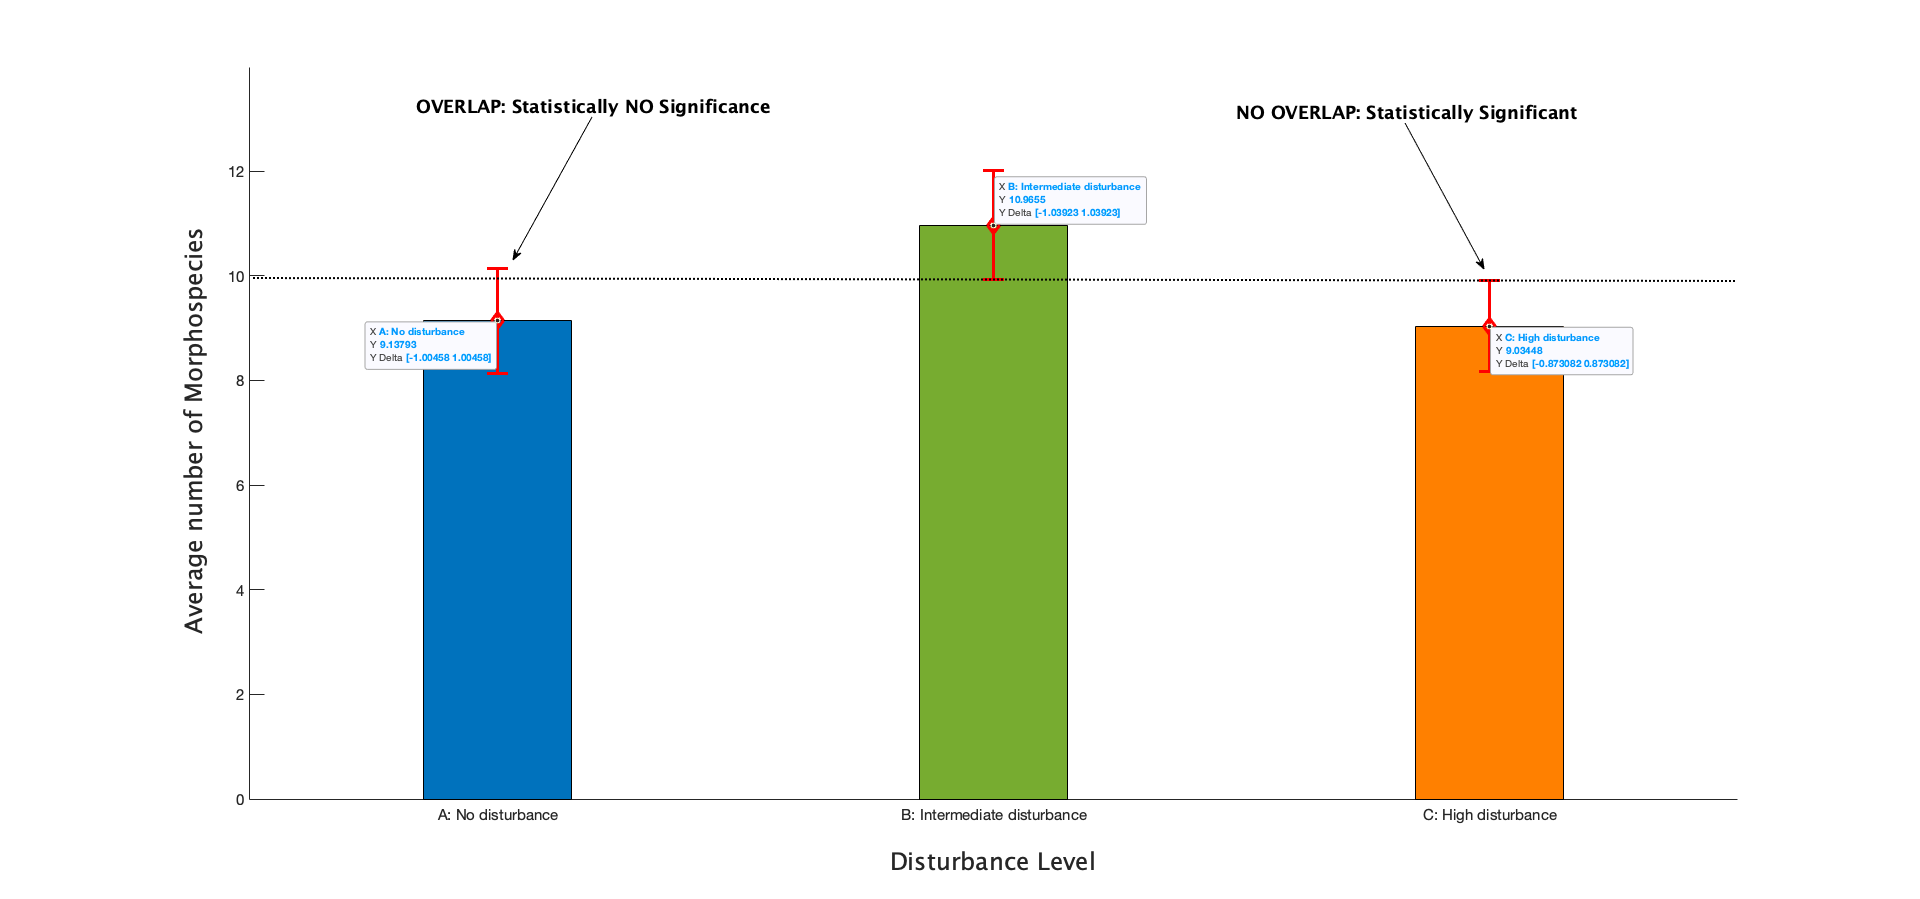
\includegraphics[width=\textwidth]{idh.png}
  \fbox{\begin{minipage}{45em}
    \begin{enumerate}
      \item What was the mean \(\pm \) standard error of coral growth (= change mg/cm2) at each of the four temperature categories?
      \begin{itemize}
        \item \C{\B{26}}: \boxed{09.82~(mg/cm^2)~\pm~0.91}
        \item \C{\O{28}}: \boxed{11.10~(mg/cm^2)~\pm~0.89}
        \item \C{\G{30}}: \boxed{13.33~(mg/cm^2)~\pm~1.04}
        \item \C{\R{26}-\R{30}}: \boxed{10.55~(mg/cm^2)~\pm~0.98}
      \end{itemize}
      \item Remember that the average water temperature of the coral's natural habitat was \C{28}. What would happen if global climate change causes the average seawater temperature to increase to \C{30}?
      \begin{itemize}
        \item
      \end{itemize}
    \end{enumerate}
  \end{minipage}}
\end{center}
\end{document}